\let\negmedspace\undefined
\let\negthickspace\undefined
\documentclass[journal]{IEEEtran}
\usepackage[a5paper, margin=10mm, onecolumn]{geometry}
%\usepackage{lmodern} % Ensure lmodern is loaded for pdflatex
\usepackage{tfrupee} % Include tfrupee package

\setlength{\headheight}{1cm} % Set the height of the header box
\setlength{\headsep}{0mm}     % Set the distance between the header box and the top of the text

\usepackage{gvv-book}
\usepackage{gvv}
\usepackage{cite}
\usepackage{amsmath,amssymb,amsfonts,amsthm}
\usepackage{algorithmic}
\usepackage{graphicx}
\usepackage{textcomp}
\usepackage{xcolor}
\usepackage{txfonts}
\usepackage{listings}
\usepackage{enumitem}
\usepackage{mathtools}
\usepackage{gensymb}
\usepackage{comment}
\usepackage[breaklinks=true]{hyperref}
\usepackage{tkz-euclide} 
\usepackage{listings}
% \usepackage{gvv}                                        
\def\inputGnumericTable{}                                 
\usepackage[latin1]{inputenc}                                
\usepackage{color}                                            
\usepackage{array}                                            
\usepackage{longtable}                                       
\usepackage{calc}                                             
\usepackage{multirow}                                         
\usepackage{hhline}                                           
\usepackage{ifthen}                                           
\usepackage{lscape}
\begin{document}

\bibliographystyle{IEEEtran}

\title{10.3.26}
\author{EE25BTECH11023 - Venkata Sai}
% \maketitle
% \newpage
% \bigskip
\maketitle 
\renewcommand{\thefigure}{\theenumi}
\renewcommand{\thetable}{\theenumi}
\setlength{\intextsep}{10pt} % Space between text and floats

\numberwithin{align}{enumi}
\numberwithin{figure}{enumi}
\renewcommand{\thetable}{\theenumi}
\vspace{-2em}
\textbf{Question:}  \\
Find the point at which the tangent to the curve $y = \sqrt{4x-3}-1$ has its slope $\frac{2}{3}$ .\\
\textbf{Solution:}  \\
Given curve
\begin{align}
y &= \sqrt{4x-3}-1 \\
y+1=\sqrt{4x-3} &\implies \brak{y+1}^2 =4x-3 \\
y^2&+2y+1=4x-3 \\
y^2&-4x+2y+4=0
\end{align}
Equation \brak{4} in matrix form
\begin{align}
y^2+2\brak{-2x+y}+4=0 \\
\vec{x}^\top\myvec{0&0\\0&1}\vec{x}+2\myvec{-2&1}\vec{x}+4=0
\end{align}
The general equation of conic
\begin{align}
    \vec{x}^\top\vec{V}\vec{x} + 2\vec{u}^\top\vec{x} + f = 0
\end{align}
On comparing \brak{6} with \brak{7}
\begin{align}
\vec{V}=\myvec{0&0\\0&1},\vec{u}=\myvec{-2\\1},f=4
\end{align}
Given slope
\begin{align}
    m=\frac{2}{3}
\end{align}
The normal vector to the given tangent is 
\begin{align}
    \vec{n}=\myvec{-m\\1} \implies \vec{n}=\myvec{-\frac{2}{3}\\1} 
    \end{align}
    \begin{align}
    |\vec{V}-& \lambda\vec{I}|=0 \\
    \mydet{\myvec{0&0\\0&1}-\lambda\myvec{1&0\\0&1}}=0 &\implies
    \mydet{\myvec{0&0\\0&1}-\myvec{\lambda&0\\0&\lambda}}=0\\
    \mydet{\myvec{-\lambda&0\\0&1-\lambda}}=0 &\implies \brak{-\lambda}\brak{1-\lambda}=0 \\
    \lambda_1=0\ &\text{and}\ \lambda_2=1
\end{align}
Finding eigen vector for $\lambda_1=0$
\begin{align}
    \brak{\vec{V}- \lambda\vec{I}}\vec{p}&=\vec{0}\\
    \myvec{-\lambda&0\\0&1-\lambda}\myvec{x\\y}=0 &\implies \myvec{0&0\\0&1}\myvec{x\\y}=\myvec{0\\0}\\
     0=0,y=0 &\implies \vec{p_1}=\myvec{1\\0}
\end{align}
For a given normal vector $\vec{n}$, the point of contact $\vec{q}$ for a given curve is given by the matrix equation
\begin{align}
\myvec{\brak{\vec{u}+\kappa\vec{n}}^\top\\\vec{V}}\vec{q}=\myvec{-f\\\kappa\vec{n}-\vec{u}} \quad\ &\text{where}\ \kappa=\frac{\vec{p_1}^\top\vec{u}}{\vec{p_1}^\top\vec{n}} \\
\kappa=\frac{\myvec{1&0}\myvec{-2\\1}}{\myvec{1&0}\myvec{-\frac{2}{3}\\1}}&=\frac{-2}{-\frac{2}{3}}=3
\end{align}
From \brak{8}
\begin{align}
\myvec{\brak{\myvec{-2\\1}+3\myvec{-\frac{2}{3}\\1}}^\top\\\myvec{0&0\\0&1}}&\vec{q}=\myvec{-4\\3\myvec{-\frac{2}{3}\\1}-\myvec{-2\\1}} \\
\myvec{\myvec{-4\\4}^\top\\\myvec{0&0\\0&1}}\vec{q}=\myvec{-4\\\myvec{-2\\3}+\myvec{2\\-1}} &\implies 
\myvec{\myvec{-4&4}\\\myvec{0&0\\0&1}}\vec{q}=\myvec{-4\\\myvec{0\\2}}
\end{align}
\begin{align}
\myvec{-4&4\\0&0\\0&1}\vec{q}&=\myvec{-4\\0\\2} 
\end{align}
Taking augmented matrix
\begin{align}
    \augvec{2}{1}{-4&4&-4\\0&0&0\\0&1&2}\xrightarrow{R_1\rightarrow R_1-4R_2}\augvec{2}{1}{-4&0&-12\\0&0&0\\0&1&2}\xrightarrow{R_1\rightarrow-\frac{1}{4}R_1}\augvec{2}{1}{1&0&3\\0&0&0\\0&1&2} 
    \end{align}
    \begin{align}
    \vec{q}=\myvec{3\\2}
\end{align}
 Hence the point of contact is $\myvec{3\\2}$
 \begin{figure}[h!]
   \centering
   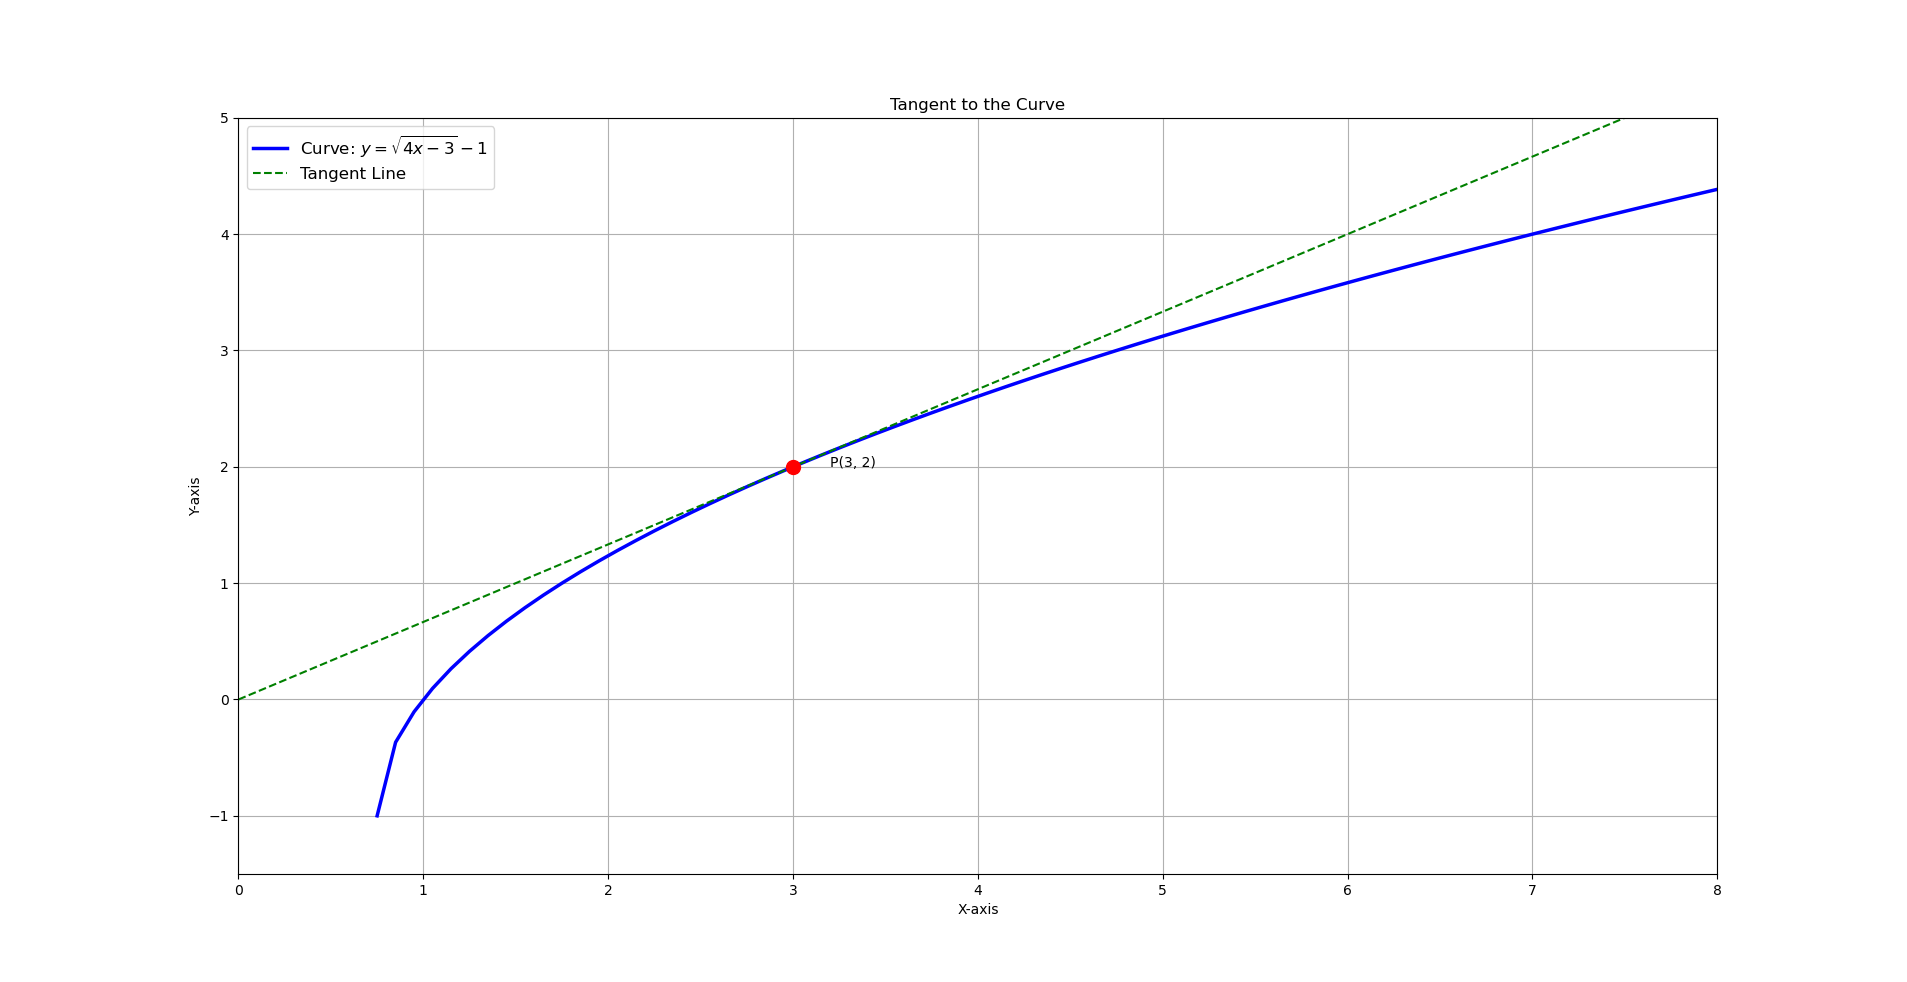
\includegraphics[width=1.\columnwidth]{figs/fig1.png}
	\caption{}
   \label{}
\end{figure}
\end{document}  
